% If you are looking for the PDF file, you can compile the .tex file or donwload the PDF from here:
% https://github.com/ilario/The_Fully_Automated_Board_Game-LaTeX

% Instruction for compiling: install TeXlive or whatever other LaTeX distribution
%
% pdflatex The_Fully_Automated_Board_Game.en
% makeglossaries The_Fully_Automated_Board_Game.en
% pdflatex The_Fully_Automated_Board_Game.en
% pdflatex The_Fully_Automated_Board_Game.en

% In order to decrease the dimension of the PDF file and reduce the resolution of some raster images, use:
% gs -sDEVICE=pdfwrite -dPDFSETTINGS=/prepress -dPrinted=false -dNOPAUSE -dQUIET -dBATCH -dAutoFilterColorImages=false -dColorImageFilter=/FlateEncode -sOutputFile=The_Fully_Automated_Board_Game-ENG-printer_quality.pdf The_Fully_Automated_Board_Game.en.pdf
% instead of preprint, you can also try /screen and /ebook

% Some rights are reserved as specified by
% Creative Commons Attribution - NonCommercial version 4.0 licence
% which can be accessed on https://creativecommons.org/licenses/by-nc/4.0/

% po4a: command -titleformat {}[]{}{}{}{}
% po4a: command -posttitle {}
% po4a: command -pretitle {}
% po4a: command -makeglossaries 
% po4a: command -date {}
% po4a: command -uppercase {_}
% po4a: command -subtitle {_}
% po4a: command -url {}
% po4a: command -texttt {_}
% po4a: command -textit {_}
% po4a: command -textbf {_}
% po4a: command -paragraph {_}
% po4a: command -newglossaryentry {}{_}
% po4a: command -glsaddall 
% po4a: command -printglossary 
% po4a: command -epigraph {_}{_}

\documentclass[a5paper, 10pt, openany]{book}

\usepackage[
    paperheight=17cm,
    paperwidth=14cm,
    top=1.3cm,
    bottom=1.3cm,
    heightrounded,
    %bindingoffset=1cm, % this is useful for keeping text away from the stapled union of the pages
    centering,
    marginparwidth=1.3cm,
    textwidth=11cm,
    marginparsep=0.1cm,
    %showframe
]{geometry}% booklets of the original box are 14x17 cm, perfectly filling the internal size of the box

\usepackage[T1]{fontenc}

\usepackage{fontawesome7} % for the rubles symbol with \faRubleSign and for the busts symbol with \faPeopleGroup

\usepackage[english]{babel}% spanish, italian, catalan, 

\usepackage{hyperref}
    \hypersetup{
        hidelinks,
        pdftitle={The Fully Automated Board Game - English rulebook},
    %        pdfsubject={Your PDF subject},
        pdfauthor={No Board Games}
        pdfkeywords={the fully automated board game, no boad games} % list of keywords
    }
    
% allowing url breaks at hyphens https://tex.stackexchange.com/a/3034/173645
% https://tex.stackexchange.com/a/407368/173645
\usepackage{xurl}

\usepackage{xcolor} % for colors in hyperref links and in thumbs
    \definecolor{colorone}{HTML}{1B9E77}
    \definecolor{colortwo}{HTML}{d95f02}
%    \definecolor{colorthree}{HTML}{7570B3}
%    \definecolor{colorfour}{HTML}{E7298A}
%    \definecolor{colorfive}{HTML}{66A61E}
%    \definecolor{colorsix}{HTML}{E6AB02}
%    \definecolor{colorseven}{HTML}{A6761D}
%    \definecolor{coloreight}{HTML}{666666}

\usepackage{glossaries} % list of explained concepts at the end of the rulebook
    \makeglossaries % has to be after glossaries and after hyperref

% automagically reduces overfull lines and improves justification, but the compilation takes longer
\usepackage{microtype} 

% for customizing titles
\usepackage{titlesec}
    % for removing "Chapter 1" from the first chapter's page
    % taken from https://tex.stackexchange.com/a/120743/173645
    \titleformat{\chapter}[display]{\normalfont\bfseries}{}{0pt}{\Huge}

% to add a subtitle. Taken from here: https://apurbapaul.blogspot.com/2013/01/subtitle-in-latex.html
\usepackage{titling}
    \newcommand{\subtitle}[1]{%
        \posttitle{%
            \par\end{center}
        \begin{center}\large#1\end{center}
        \vskip0.1em}}%
    
    % bigger main title
    \pretitle{\begin{center}\Huge}

    \posttitle{\par\end{center}\vskip 0.5em}

% to add the colorful marks on the page edges
\usepackage[width=1cm]{thumbs}

% electronic pdf bookmark, no change in the printed version
\usepackage{bookmark}

\usepackage{epigraph}% for inserting stupid phrases in random places
%\setlength{\epigraphrule}{0pt}% eliminate the rule below the epigraphs
    
\usepackage{rotating} % for vertical sideways text


% limit main table of content to sections, do not print subsections
\setcounter{tocdepth}{1}

% we don't want to show the 1.2.3 numbering before the section titles, but we still want them to appear in the table of contents
% using \section*{} removes the numbering but also removes them from the ToC
% solution taken from https://tex.stackexchange.com/a/11669/173645
\setcounter{secnumdepth}{0}

\author{No Board Games}
\date{2025}


\title{\uppercase{The Fully Automated\\ Boardgame}\\
    English rulebook
    % the poster image in the title page, idea taken from here:
    % https://tex.stackexchange.com/a/551584/173645
    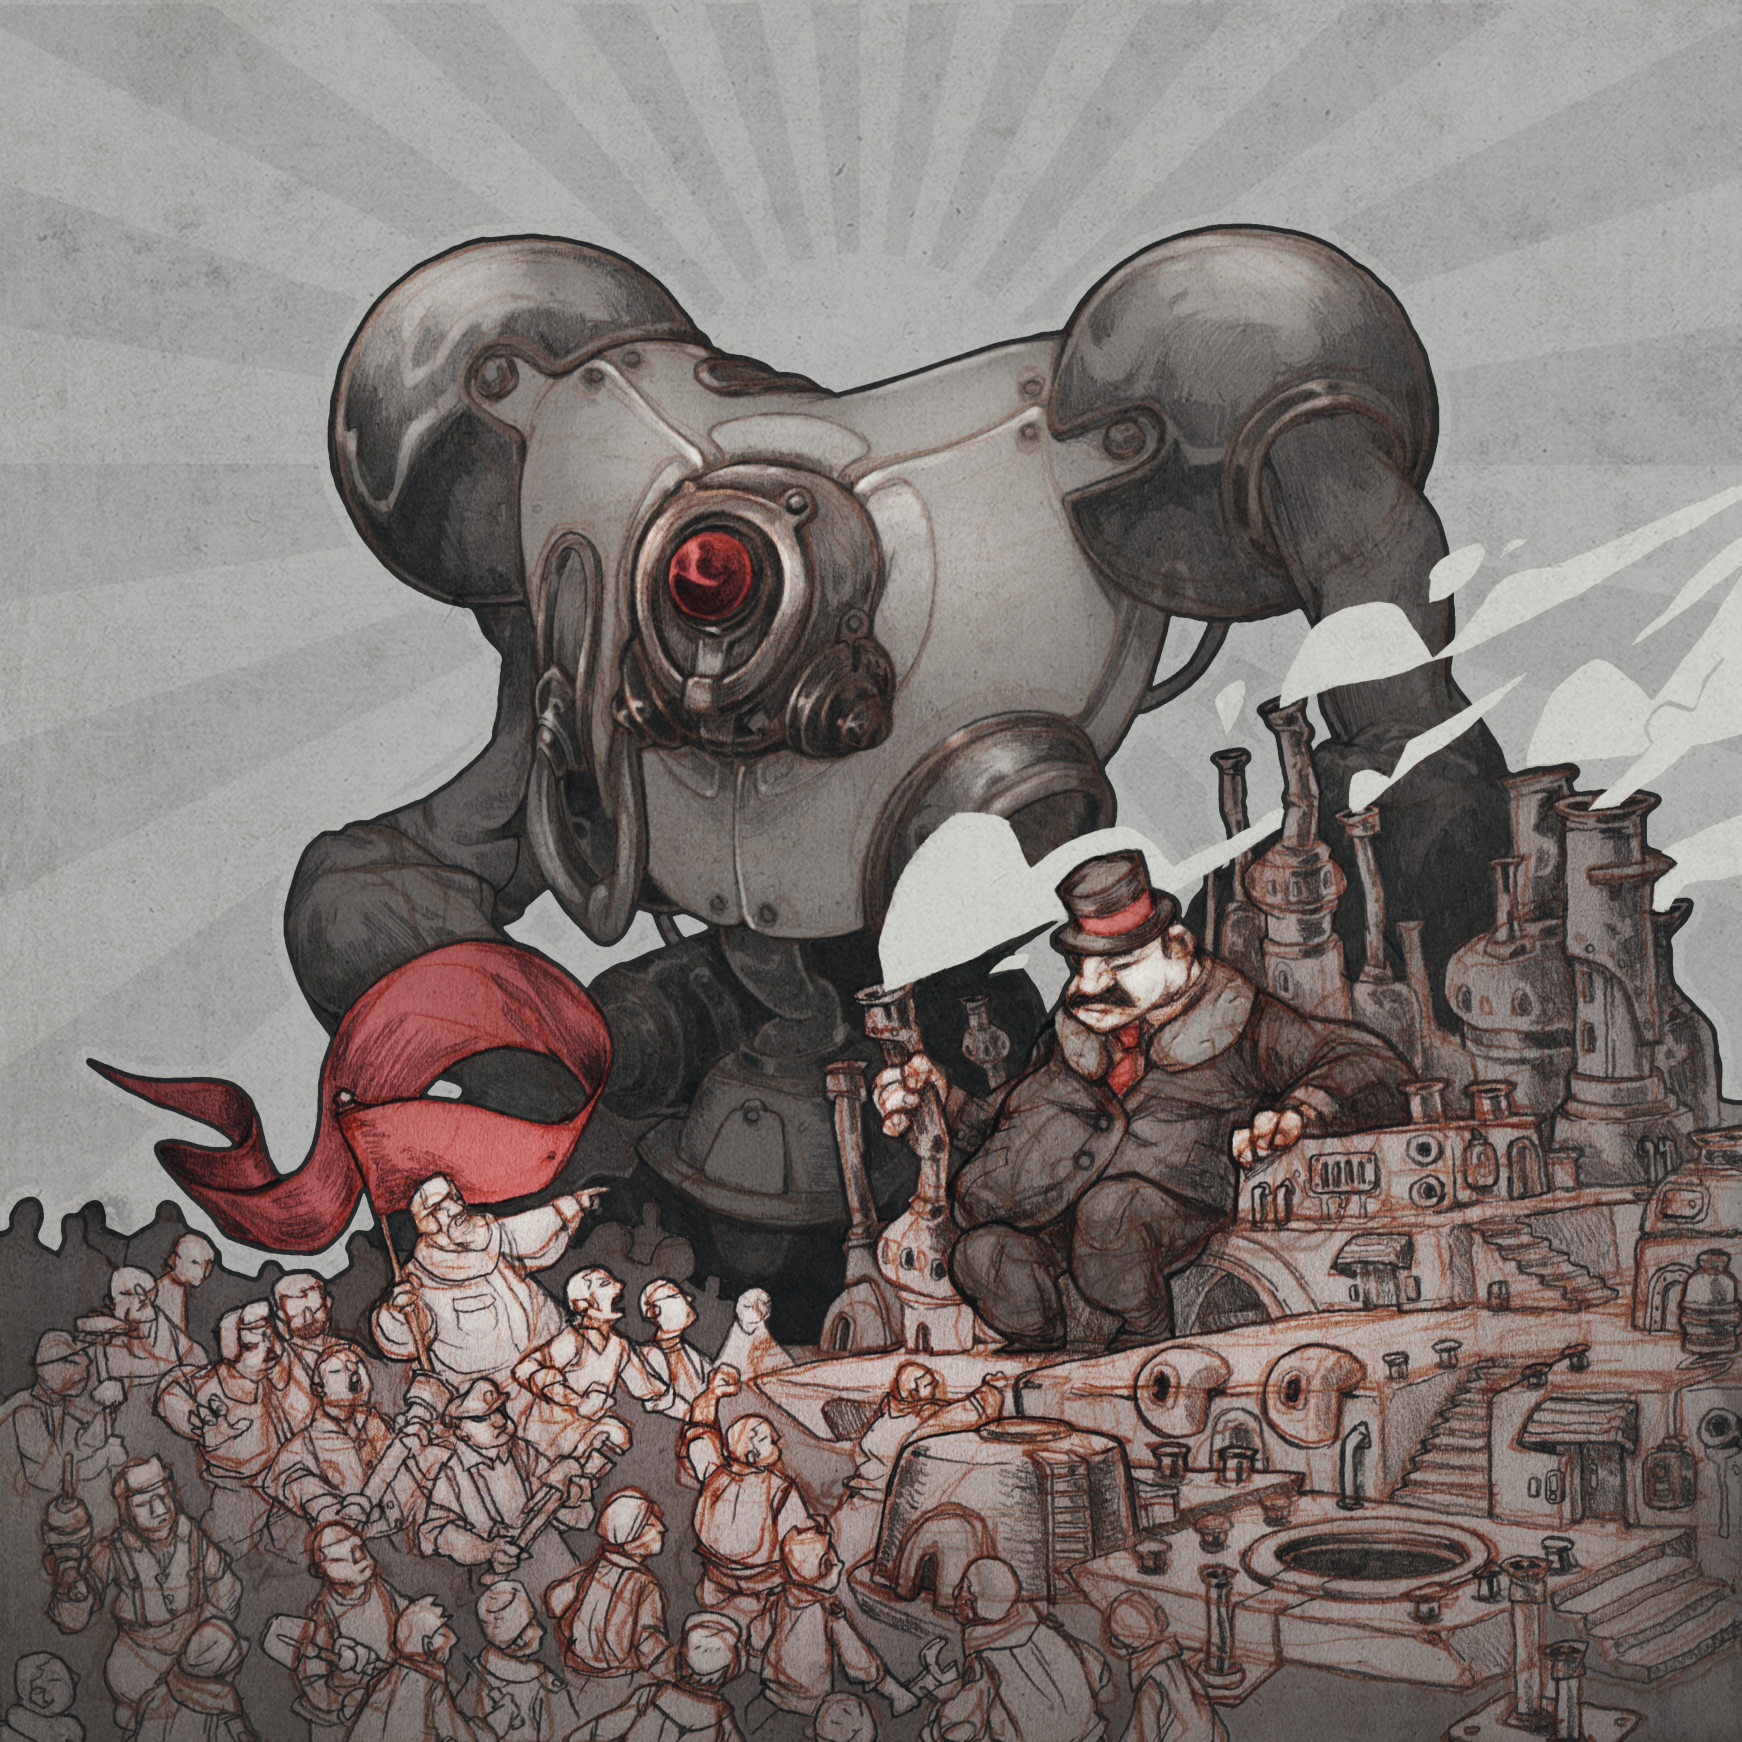
\includegraphics[scale=0.47]{cover.jpg}}

\subtitle{A party game about robots and strikes.\\
    Become a greedy boss or a riotous worker!
    
    ---
    
    From 2 to 10 players\\
    Duration 1 to 60 minutes}

\begin{document}

\selectlanguage{english}

\maketitle

\tableofcontents

\mainmatter

% Some rights are reserved as specified by
% Creative Commons Attribution - NonCommercial version 4.0 licence
% which can be accessed on https://creativecommons.org/licenses/by-nc/4.0/

Copyright 2025 No Board Games
% closing the group opened for avoiding the page break after the ToC

\endgroup

Some rights are reserved as specified by Creative Commons Attribution - NonCommercial version 4.0 licence, which can be accessed on

\url{https://creativecommons.org/licenses/by-nc/4.0/}

\vfill

\begin{minipageparindent}{0.8\linewidth}
    \textbf{No Board Games} is an international group that creates radical board games.
    Check for gameplay videos on our website: \url{https://noboardgames.com}
\end{minipageparindent}%
%\hfill
\begin{minipage}{0.2\linewidth}
    
\includegraphics[width=1\textwidth]{QR_code_NoBG.png}
\end{minipage}

\vfill

\begin{wrapfigure}[6]{R}{0.23\textwidth}
    \vspace{-0.5cm}
    \centering
    
\includegraphics[height=6\baselineskip]{QR_code_BGG_forum.png}
\end{wrapfigure}

\textit{You are reading the version 1.0 of the rulebook, printed in English and Italian. For new
revisions and more translations, check our website. If you want to contribute translations,
contact us at: info@noboardgames.com
The development and discussion on the rules will continue on BoardGameGeek forum
"Rules". Log your games on the forum "Sessions".} \url{https://boardgamegeek.com/boardgame/357812/fully-automated-board-game/forums/}

Printed in Poland by Fabryka Kart, 2025.

\section{ACKNOWLEDGEMENTS}

    \textbf{Design}: Matteo Modena, Ilario Gelmetti
    
    \textbf{Art}: Bernardo "RUPE" Anichini - IG: \texttt{@rupe\_b}
    
    \textbf{Testing}: Ilario Gelmetti, Matteo Modena, Matteo Paolini, Giulio Mazzocchi,Bernardo Anichini,
    Emanuele Croce, Dan Howitt, Luis Gutiérrez, Nicola Fiorillo, Loz, Riccardo Bernori,
    Luna Golino, Michele Bertoldi
    
    \textbf{Communication}: Matteo Paolini, Matteo Modena
    
    \textbf{Video}: Davide Morittu
    
    We want to thank all the backers that trusted us during the crowdfunding campaign, and
    specifically "The Boss" backers: \textbf{Rock Castle}, \textbf{Matteo R.} and \textbf{Comrade Alex}!
    
    Also, this game would not have been possible without the countless online testing
    sessions that were joined by many. Special thanks go to the heroic \textbf{Dan Howitt} and the
    unstoppable \textbf{Luis Gutiérrez}.


\section{BACKGROUND}

    \epigraph{The working class and the employing class have nothing in common.}{\textit{Industrial Workers of the World}}
    
    There will never be peace between the oppressed and the oppressors, and thus between
    master and subordinate. From the first utopian socialists to the present day, a new vision
    of social change has emerged, one based on class struggle. The employers have acquired
    their wealth on the systematic exploitation of the working class, leveraged technology to
    fuel this mechanism, and for avoiding strikes and sabotage. Faced with new technologies,
    capable of speeding up and improving the efficiency of production, some have responded with
    sabotage and destruction, such as the Luddite movement*, and those who
    have claimed all the benefits, such as the Left-wing Accelerationist movement. This game
    encourages you to confront the question of the automation of work, the ever decreasing
    need of wageworkers, and, more generally, with the concept of class struggle. Because
    there will always be class struggle as long as power and resources are not distributed
    equally among people.
    
    \textsl{*The Luddite movement was a class struggle in England during the 19th century, whereby
    workers struggled against their labours being replaced with machinery.}


\section{OVERVIEW}

    Take the role of a greedy boss (representing the Bourgeoisie) or suffer the burden of a
    worker (representing the Proletariat).
    
    As a \textbf{worker}, you must negotiate and accept Contracts from the bosses, to collect enough
    coins to pay your Rent and \textbf{survive}. But only a collective and coordinated \textbf{strike} will bring
    victory to the workers.
    
    As a \textbf{boss}, you control the production, the money, and therefore the workers. You must
    offer the favoured Contracts and \textbf{accumulate the greatest profit} before your competitor
    does.
    
    The Fully Automated Board Game is a fusion of negotiation, hidden roles, bluffing, voting,
    and class struggle.


\section{COMPONENTS}


    \subsubsection{PHASE MARKER TOKEN}
        \begin{wrapfigure}[7]{R}{0.23\textwidth}
            \vspace{-0.5cm}
            \centering
            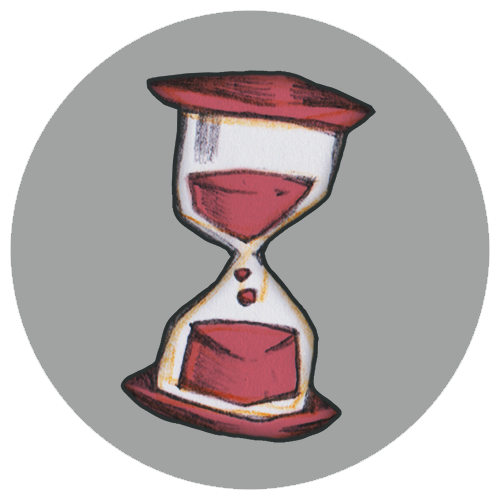
\includegraphics[height=6\baselineskip]{token_phase.jpg}
        \end{wrapfigure}
        In this box, we decided to not include any component representing
        the \faRubleSign\ money. Instead, we propose
        you to use real coins. This will make
        the gameplay feel more "real" and
        allows us to reduce the materials,
        thus making the box smaller, more
        portable, and its fabrication less
        polluting. For the same reason, this
        game has been fabricated with the
        eco-friendly materials and methods of Fabryka Kart in Poland.
        At the end of each game session,
        we encourage you to take all the
        real coins used as in-game currency and make a donation to a
        union or a social project, in the real
        world! Consider this a way of helping your local social community.
        Reach out, maybe we can recommend some entity!

    \subsubsection{WHAT'S IN THE BOX}
        \begin{multicols}{2}
            \begin{itemize}
                \item 2 Boss cards - Bourgeoisie
            (blue card with a blue pig symbol)
            
                \item 10 Worker character cards:
            
                \begin{itemize}
                    \item 4 Proletarians - Virtual pauper
            (red card with a red flag symbol)
            
                    \item 3 Startupper - Petite bourgeoisie
            (red card with a blue pig symbol)
            
                    \item 2 Scab - Workaholic (red card with a
            symbol of a mug "I \textless3 Mondays")
            
                    \item 1 Luddite - Saboteur
            (red card with a bomb symbol)
            \end{itemize}
            
                \item 10 Robot cards (blue and red sides)
                \item 17 Event cards
                \item 6 Contracts cards
                \item 1 Union Fund card
                \item 1 Public Work card
                \item 1 Mayor card
                \item 1 Security Guard card
                \item 6 Phase cards
                \item 8 Personal tokens for workers
                \item 1 Phase marker token
            \end{itemize}
        \end{multicols}


\chapter{Rules for 5 to 10 players}\label{ch:5-10}

    \addthumb{\thechapter}{\begin{sideways}\large{\textbf{5-10 \faPeopleGroup}}\end{sideways}}{white}{colorone}

    % Some rights are reserved as specified by
% Creative Commons Attribution - NonCommercial version 4.0 licence
% which can be accessed on https://creativecommons.org/licenses/by-nc/4.0/

\section{NUMBER OF PLAYERS}

    \textbf{Beware!} The rules of the 5–10 \faPeopleGroup\ game are very different from the ones for 2–4 \faPeopleGroup! \textbf{Some
    cards have a text saying} "5–10 \faPeopleGroup": this is the side to use for games from 5 to 10 players.



\section{SET-UP}

    \begin{enumerate}
        \item Take the role cards following the table, shuffle and hand out one card face
        down to each player. \textbf{Two} players will have the \textbf{boss} role and the \textbf{rest will
        be workers}.
        \item Each worker should check the \textbf{role} but \textbf{keep it secret}.
        \item Give a \textbf{personal token} to each worker. Try to find the best suited token for
        each person, so that the association will be easier to remember. Keep aside
        the hourglass token.
        \item Place the \textbf{Robots} (stacked), \textbf{Public Work}, \textbf{Union Fund}, \textbf{Mayor}, and \textbf{Security
        Guard} cards at the centre of the table.
        \item Place the 6 \textbf{phase cards} (on the "5–10 \faPeopleGroup" side) face up one next to the other
        at the centre of the table. Place the \textbf{phase marker token} (the one with an
        hourglass drawing) on the first phase card.
        \item Create a space for the \textbf{Bank} where you put a \textbf{pile of coins}. Take plenty of
        coins, the exact amount is not important (for a 5 \faPeopleGroup\ game, you will need
        approximately 60 coins representing 60 \faRubleSign). Use some real coins, if you have
        them, for representing the \faRubleSign, the in-game currency. If you don't have coins at
        hand, you can use anything you "borrowed" from work or any other small and
        homogeneous object you can find. Alternatively, take note of the amount of
        coins on a piece of paper.
        \item Each \textbf{Boss starts with 10 \faRubleSign}\ coins, and workers with 0 \faRubleSign.
        \item The two halves of the game box can be handed to the bosses for covering
        and keeping their amount of coins secret.
        \item The bosses decide which activity they want to compete over. In the spirit of
        the game, players are encouraged to \textbf{role-play from this point on}, starting with each boss
        announcing the name of their company and their unique
        winning business model.
    \end{enumerate}

    \subsubsection{EXAMPLE}

        \itsmall{The bosses decide they will compete in the production of spicy watermelon-flavoured
        toilet paper. Boss X asserts that "Hot bottom roots" will be successful as
        their product is sustainable, because it embeds watermelon seeds in the paper. Boss
        Y defends that the patented idea of having triangular shaped paper will crush the
        competition, making "Rusty nachos" the most used toilet paper worldwide.}



\section{VICTORY CONDITIONS}

    Whoever achieves the \textbf{victory} conditions, \textbf{at any moment}, can declare victory,
    and end the game. It can happen for more than one player at the same time. In
    this case, all these players win the game.

    \subsection{BOSS' VICTORY}
    
        \textbf{A boss wins when reaching a certain amount of coins.}
    
    \subsection{WORKERS COLLECTIVE VICTORY}
    
        \textbf{All the workers win collectively} when they manage to achieve full automation,
        meaning they manage to \textbf{expropriate as many robots as the number of workers}.
        For games with at least 6 \faPeopleGroup, when a Luddite role is present, the robots destroyed
        by the Luddite also count towards the workers' collective victory.
        After an epic victory, the players are encouraged to collect all the metallic coins
        used for playing and use them for making a donation to a workers' union or social
        movement. In the real world! We mean, out of this game, give those pennies some
        real use!
    
    \subsection{STARTUPPERS' VICTORY}
    
        The worker with the \textbf{Startupper} secret role can win with \textbf{workers' collective victory}
        conditions or \textbf{individually} with a \textbf{Class Betrayal}: Accumulating \textbf{as many
        coins as the total number of players} (workers + 2 bosses). The Startupper \textbf{cannot} declare
        the individual victory \textbf{while Stressed}. Also, for reaching the needed
        amount of cash, the Startupper can \textbf{steal} all the coins from the \textbf{Union Fund} card.
        The Startupper victory (the victory of the small-medium enterprise) means that a
        worker earns a lot and opens a new business!
    
    \subsection{SCABS' VICTORY}
    
        Each \textbf{Scab} can win with \textbf{workers' collective victory} conditions or \textbf{together with
        a boss}: when a boss declares victory, the Scab also wins \textbf{if has been working} (not
        striking!) \textbf{for that boss} in the same turn (regardless if the Scab is Stressed or not).
    
    \subsection{LUDDITE'S VICTORY}
    
        [6–10 \faPeopleGroup.] The \textbf{Luddite} can win with \textbf{workers' collective victory} conditions
        (counting all the expropriated and the destroyed robots) or \textbf{individually}. The
        individual victory happens for the Luddite as soon as \textbf{3 robots get destroyed}. To
        understand how robots can be destroyed by the Luddite, see what happens in a
        failed strike during phase 2 "Strike".
    
    \subsection{EARLY ENDING OF THE GAME - MONOPOLY}

        \textbf{If a boss is eliminated} from the game (i.e. cannot pay Rent, or cannot buy a
        robot after a successful Acceleration Strike held by the workers), a \textbf{Monopoly} is
        formed by the other boss. The workers immediately and automatically expropriate
        the robots of the bankrupted boss.
        In a Monopoly situation, the winner gets determined based on the \textbf{number of
        robots controlled by the workers}:

        \begin{enumerate}
            \item If the workers have at least as many robots (expropriated or destroyed by the
            Luddite) as half of the number of workers (rounded up), they collectively win
            (i.e. 3 workers with 2 robots, 4 workers with 2 robots...);
            \item Otherwise, the surviving boss wins.
        \end{enumerate}

\section{GAMEPLAY}

    The game is played in rounds until 1 or more players achieve their victory conditions.
    When this happens, the game immediately ends.
    A round consists of \textbf{6 phases}. Each phase is played a little differently; there is no
    player turn order, and the actions of bosses or workers can take will differ.

    \begin{itemize}
        \item \textbf{Phase 1 HIRING}: bosses compete for workers by offering Contracts; and
        may acquire robots to bolster production. Workers must choose a Contract.
        Players can discuss openly and negotiate.
        \item \textbf{Phase 2 STRIKE}: bosses may compete for the Security Guard. Each worker
        must decide to work or to strike. Players can discuss intentions, but must
        decide and then reveal their actual action during a simultaneous vote.
        \item \textbf{Phase 3 PRODUCTION}: bosses gain coins from the Bank, equal to the production
        or their workers and robots.
        \item \textbf{Phase 4 PAYDAY}: bosses may pay their workers' salaries.
        \item \textbf{Phase 5 RENT}: both bosses and workers pay their Rent.
        \item \textbf{Phase 6 UNION FUND}: workers may place their coins into the shared Union
        Fund.
    \end{itemize}



\section{Phase 1 HIRING}

    \subsection{BOSSES ACTIONS}
    
        \begin{itemize}
            \item \textbf{May acquire} as many \textbf{robots} as they are able to; return 6 \faRubleSign\ coins to the Bank
            (the pile of no one's coins) and place 1 robot in front of them, blue side face
            up.
            \item Must outline their \textbf{Contract offers} - in return for work, how many coins will
            Workers receive. Contracts are \textbf{not binding}. Contracts can be verbal or written,
            the role playing is up to you.
            \item \textbf{Holidays}: in addition to a salary, Contracts may include Holidays. This does
            not have an extra cost for the boss. During phase 4 Payday, Holidays allow
            workers to \textbf{eliminate Stress}. To understand how workers can get Stressed,
            see phase 5 Rent.
        \end{itemize}
        
    \subsection{WORKERS ACTIONS}
    
        \begin{itemize}
            \item May attempt to negotiate with the bosses for better pay.
            \item Must \textbf{pick who they will work for} by giving a boss their personal token.
            \item Depending on the number of players, at most [5–6 \faPeopleGroup] one, or [7–8 \faPeopleGroup] two,
            or [9–10 \faPeopleGroup] three workers may \textbf{alternatively perform Public Work}, by placing their
            personal token on the Public Work card.
            \item \textbf{Public Work} provides some workers (max. 1, 2, or 3 depending on the number
            of players), with a Contract for a \textbf{single round}, paying \textbf{1 coin} with \textbf{included Holidays}.
        \end{itemize}
            
    \subsection{ADDITIONAL DETAILS AND EXAMPLES}
    
        \begin{itemize}
            \item Contracts given to workers can pay 0, up to anything a boss determines.
            Contracts can include promises of future pay increases. Contracts given to
            individual workers can differ. Role playing/creativity when giving out Contracts is encouraged!
        \end{itemize}
    
        \subsubsection{EXAMPLE}
        
            \itsmall{Boss X offers one Contract for 2 \faRubleSign\ and one internship Contract starting from 0 and increasing
            by 1 coin each round. Boss Y returns 6 \faRubleSign\ to the Bank to purchase 1 robot. And offers three
            Contracts for 1 coin. Diana, the Luddite, rushes to take the only 2-coins Contract, giving her
            personal token to boss X. Caino, the Startupper, takes the Public Work, placing his player
            token on the Public Work card. As there are 6 players (2 bosses + 4 workers) there is only 1
            Public Work job available. Beata, the Scab, believes in meritocracy and trusts boss X, so takes
            the internship Contract. Abele, the Prolet, takes one of the 1-coin Contracts from boss Y.}



\section{Phase 2 STRIKE}

    \subsection{BOSSES ACTIONS}
    
        \begin{itemize}
            \item \textbf{Must bid for the Security Guard}, even if their bid is 0, \textbf{using fingers} to
            indicate a number from 0 to 5 \textbf{during the simultaneous voting}.
        \end{itemize}
        
    \subsection{WORKERS ACTIONS}
    
        \begin{itemize}
            \item \textbf{All non-Stressed workers} must decide to strike or work; using, \textbf{during the
            simultaneous voting}, a \textbf{closed fist to strike or an open hand to work}.
        \end{itemize}
    
    \subsection{ALL PLAYERS}

        \begin{itemize}
            \item \textbf{Simultaneous voting}: all the bosses and the non-Stressed workers place
            their hands in the centre of the table, then \textbf{simultaneously reveal their action}.
        \end{itemize}
    
    \subsection{VOTE RESOLUTION}

        \begin{itemize}
            \item First thing after the vote, \textbf{both bosses pay} to the Bank an amount of coins
            equal to \textbf{their bid multiplied by the number of robots} each of them controls.
            For example: if a boss has 2 robots and indicated the number 3 with
            the fingers, will have to pay 6 to the Bank. If the boss has no robots, they will
            simply pay the bid amount, like if she had 1 robot.
            \item The winner of the bidding is the boss with the \textbf{highest bid}: the one who
            indicated the highest number \textbf{with the fingers}, regardless the actually paid
            amount.
            \item \textbf{Security Guard card}: then, the boss who won the bidding, receives the Security
            Guard card for this round. This \textbf{protects} this boss from \textbf{Expropriation
            Strike and Sabotage}. It does not protect against Acceleration Strike.
            \item If both bosses bid the same amount with the fingers, neither receives the
            Security Guard, yet both have to pay.
            \item For a \textbf{strike to be successful}, the \textbf{majority of workers} must take the \textbf{strike
            action} (e.g. with 4 workers, 3 workers must strike). In case of tie (i.e. 2 out of
            4 workers striking) or when just a minority strikes, the strike fails. For calculating
            the required majority, also the Stressed workers are considered (e.g. with
            4 workers in total, if 2 are Stressed it is impossible to reach the majority, as
            the Stressed ones cannot strike).
            \item \textbf{Failed Strike}: [5 \faPeopleGroup] In absence of the Luddite role, nothing happens, simply
            the striking workers will not produce during phase 3 Production. [6–10 \faPeopleGroup]
            The \textbf{Luddite could attack}! If at least two workers participated in a failed
            strike (which did not reach the majority) and there is at least one robot in the
            game (either associated to a worker or owned by a boss but not protected
            by the Security Guard card), the bosses close their eyes and both count down
            aloud from 10. At this moment, if the Luddite was one of the participants
            of the failed strike, \textbf{may destroy one robot} (either assigned to a worker or
            owned by a boss, unless the Security Guard is protecting it). The Luddite can
            take the robot card and put it in a robots' rubbish pile (any place on the table,
            just make clear that this robot is not assigned to any player). The destroyed
            robots won't produce coins for anyone, but will count towards the workers'
            collective victory condition together with the expropriated robots. Also, destroying
            robots helps the Luddite to achieve an individual victory: If 3 robots
            get destroyed (over 3 failed strikes), see Luddite's victory conditions.
            \item If a \textbf{strike} is \textbf{successful}; workers involved must collectively \textbf{decide} to \textbf{Expropriate}
            a robot or \textbf{Accelerate} the acquisition of a robot. If the workers cannot
            agree on what type of strike they want to carry out, then the bosses decide.
            \item \textbf{Expropriation strike}: workers \textbf{take a single blue robot owned by a boss}
            (excluding the boss whose robots are protected by the Security Guard), flip
            the card to the red side and \textbf{assign it to a single worker}. If the workers
            cannot agree on who keeps the robot, the bosses choose which worker will
            receive it.
            \item \textbf{Acceleration strike}: forcing a single \textbf{boss to purchase a blue robot} instantly,
            paying its cost immediately (6 \faRubleSign). This robot remains in control of the boss.
        \end{itemize}
    
    \subsection{ADDITIONAL DETAILS AND EXAMPLES}

        \begin{itemize}
            \item \textbf{Stressed workers cannot strike} and so must work.
            \item The non-Stressed workers who took the Public Work, if any, can strike but
            would receive neither the related 1-coin salary nor the free Holidays.
            \item \textbf{Workers who strike will not produce} during phase 3 Production for their
            boss, regardless if the strike was successful or not.
            \item At the end of this phase, return the Security Guard card to the centre of the
            table.
        \end{itemize}

        \subsubsection{EXAMPLE: Security Guard}

            \itsmall{During the simultaneous voting, boss Y bids 1 with one finger, supposing that it will
            be enough for protecting their shiny new robot. But boss X, evil in nature, also bids
            1, even without having any robot to protect! As they both bid the same, nobody
            gets the Security Guard and boss Y's shiny robot is unprotected, exactly what boss
            X was hoping for. Even if nobody got the Security Guard, both bosses have to pay.
            Boss Y pays their bid of 1 multiplied by 1 (1 robot): for a total of 1. This mastermind
            move will not be free for boss X: They control no robots but must still pay their bid
            of 1.\newline
            ... in a later round, boss X has 1 robot and bids 3, while boss Y has 2 robots and bids
            2. In this case, boss X pays 3 to the Bank, boss Y pays 4 (2 multiplied by 2 robots).
            Boss X is protected by the Security Guard (Boss X bid higher, despite boss Y paying
            more).}

        \subsubsection{EXAMPLE: Strike}

            \itsmall{At the same time of the bosses' bidding, the workers' vote happens. Abele, Caino,
            and Diana, in an optimism surge, close their fists to indicate that they are striking,
            while Beata keeps it open and goes to work. With 3 participants, the majority of
            the workers' is secured and the strike is successful. At this point, Abele, Caino and
            Diana can decide to Accelerate (force one boss to buy a robot immediately) or to
            Expropriate one of the robots a boss already owns. They decide to take one of the
            robots from boss Y, that are not protected by the Security Guard. Caino the Startupper
            asks Abele and Diana if he can keep the robot, they have nothing against this
            and they accept.}

        \subsubsection{EXAMPLE: Sabotage}

            \itsmall{[6–10 \faPeopleGroup: the Luddite role is present] ... the next round, boss X has 1 robot and again
            manages to get the Security Guard, and boss Y also has 1 robot. At the same time
            as the bosses' bidding, the workers reveal their votes: Abele the Prolet and Diana
            the Luddite close their hands in a fist (they strike), while Beata keeps her hand open
            (she works). Caino has to go to work, as he got Stressed in the previous round (he
            couldn't pay the Rent in phase 5). So, only two workers over four are striking, not
            reaching the majority needed for proceeding to a strike. Even if the strike failed, the
            Luddite (a secret role for games with at least 6 \faPeopleGroup) can still do things! The bosses
            close their eyes and, aloud, count back from ten. In a rage, Diana the Luddite destroys
            boss Y's robot and swiftly moves boss Y's blue robot card to the centre of the
            table. Now the workers are one robot closer to the workers' collective victory, but
            the Luddite is also closer to an individual victory!}



\section{Phase 3 PRODUCTION}

    \subsection{BOSSES ACTIONS}

        \begin{itemize}
            \item Each \textbf{robot and non-striking worker produces 5 \faRubleSign}\ for their boss. Each boss
            gains coins from the Bank equal to the total production of their workers and
            robots.
        \end{itemize}

    \subsection{WORKERS ACTIONS}

        \begin{itemize}
            \item Each \textbf{expropriated robot produces 1} coin for the worker it is assigned to;
            gain coins from the Bank equal to total production.
        \end{itemize}
    
    \subsection{ADDITIONAL DETAILS AND EXAMPLES}

        \subsubsection{EXAMPLE}

            \itsmall{Boss X has 1 robot producing 5 and a Contract with Beata who also produces 5.
            Abele and Diana went on strike, so they don't produce. Caino's robot produces 1.
            Boss X gains 10 \faRubleSign; boss Y gains no coins; and Caino gains 1 coin.}


\section{Phase 4 PAYDAY}
    
    \subsection{BOSSES ACTIONS}

        \begin{itemize}
            \item Decide on \textbf{whether or not to pay their workers} as promised in the Contracts
            given. Each boss can decide whether to distribute the salary as promised,
            keep it with an excuse, pay it only in part, or keep promises with some
            worker/s and not with others. Most likely, whoever went on strike will not
            receive any salary. Also, if an offered Contract includes Holidays, the boss
            may remove the worker's Stress for free (Untap the character card).
        \end{itemize}
    
    \subsection{WORKERS ACTIONS}

        \begin{itemize}
            \item Each worker who took the \textbf{Public Work} (if any) and did not strike, earns \textbf{1
            coin} and receive \textbf{free Holidays}.
            \item Also, each Stressed worker can \textbf{pay for their own Holidays} by giving \textbf{2 \faRubleSign}\ to
            the Bank. They may take this from their own money and/or from the Union
            Fund card (see phase 6 Union Fund).
            \item \textbf{Holidays} allow workers to \textbf{remove their Stress}. To understand how workers
            can get Stressed, see phase 5 Rent. To remove the Stress, \textbf{Untap the character
            card}, placing it straight in front of the player.
        \end{itemize}
    
    \subsection{ADDITIONAL DETAILS AND EXAMPLES}

        \begin{itemize}
            \item The \textbf{Mayor} is a \textbf{prize lasting one round}. Initially, it is placed at the centre
            of the table, not assigned to any boss/worker. It goes to the boss who \textbf{has
            at least one working} (non-striking) \textbf{worker}, \textbf{respects all the Contracts} (excluding
            the striking workers' Contracts), and \textbf{pays at least 1 coin} to each
            working worker. If only one boss respects these conditions, the Mayor card
            goes to this boss, and will be very useful for dealing with the Rent in phase
            5. If no boss deserves it, and at least one worker worked (didn't strike) for
            a boss (not for the Public Work), then one of the workers becomes the new
            Mayor (workers decide whom). Otherwise, if both bosses deserve it, or if no
            boss deserved it and no worker actually worked for any boss (so no boss had
            the possibility to respect the Contracts), then nobody gets the Mayor card.
        \end{itemize}
    
        \subsubsection{EXAMPLE}

            \itsmall{Caino was Stressed, and worked for the Public Work, so he gets directly 1 coin and
            free Holidays, which means he is not Stressed any more and Untaps his character
            card. Beata worked for boss X, and asks for her 1-coin salary. But boss X had to gift
            to the firstborn a submarine trip for seeing the Titanic, and cannot spend more this
            month, apologizes follow. Abele and Diana, as they participated in a strike (even
            if a failed one) do not receive any salary. Boss Y had only an employee, Abele, but
            he went on strike, so boss Y cannot get the Mayor card (didn't have at least one
            working worker). Boss X had a Contract with Beata and another with Diana. Diana
            participated in a strike, so she is not relevant for deciding on the Mayor card. Beata
            instead went to work, yet her salary has not been paid. If her salary had been paid,
            boss X would have got the Mayor card. So, no boss deserves to be the Mayor, and
            Beata actually worked for boss X. This means that the Mayor card goes to a worker.
            Everybody considers that Beata deserves it, so she gets elected as the new Mayor!\newline
            [...] the next round, only Caino accepted to work for boss X with a 1-coin salary.
            Unexpectedly, boss X respected the Contract and paid him 1 coin. Boss Y was hit by
            a mass strike instead, and didn't even have the option to pay the workers. Thanks
            to the gained trust, boss X becomes the "lesser evil" and gets elected as the new
            Mayor.}



\section{Phase 5 RENT}

    \subsection{BOSSES ACTIONS}

        \begin{itemize}
            \item Each \textbf{boss} must \textbf{pay} a Rent of \textbf{2 \faRubleSign}\ to the Bank.
        \end{itemize}
    
    \subsection{WORKERS ACTIONS}

        \begin{itemize}
            \item Each \textbf{worker} must \textbf{pay} a Rent of \textbf{1 coin} to the Bank.
        \end{itemize}
    
    \subsection{ALL PLAYERS}

        \begin{itemize}
            \item The player, worker or boss, who has the \textbf{Mayor card}, if any, can indicate
            \textbf{which players} (just one, some of them, or all) \textbf{will not pay} any Rent for this
            turn (herself/himself included). Additionally, this player can also \textbf{increase the
            Rent by 1 coin for one player} for this turn.
        \end{itemize}
    
    \subsection{ADDITIONAL DETAILS AND EXAMPLES}

        \begin{itemize}
            \item \textbf{If any worker cannot pay} the Rent:
            \begin{itemize}
                \item They may use the coins on the \textbf{Union Fund} card for paying the
                Rent;
                \item If there are no coins on the Union Fund card, the workers who cannot
                pay \textbf{get Stressed}: these players Tap (rotate 90 degrees) their character
                card. A Stressed worker cannot strike, so in phase 2 will have to go to
                work.
                \item Any worker that has no coins and is already Stressed, just stays like
                that, without paying the Rent.
            \end{itemize}
            \item \textbf{If a boss cannot pay the Rent}, see \textbf{Early ending of the game - Monopoly}.
            \item At the end of this phase, return the Mayor card to the centre of the table.
        \end{itemize}
    
        \subsubsection{EXAMPLE}

            \itsmall{As the new Mayor, the first law issued by boss X is to close down the fine arts museum
            in order to limit public spending. The second law, assigned the same museum
            to be the new house of the Mayor. With an act of charity, boss X allows Caino, the
            most loyal of the workers, to be the housekeeper. So, neither boss X nor Caino will
            have to pay the Rent for this round. Additionally, the new Mayor declares a central
            street to be a new space for freedom of expression, allowing any kind of street artist
            to perform there, day and night. Obviously, the residents will have to contribute
            with the initiative, like paying the paint for the graffiti artists. Fortuitously, that's
            where boss Y resides, so boss Y's Rent will be raised to 3 \faRubleSign\ for this round.\newline
            [...] the next round, Diana had some savings, and even after participating in two strikes
            can still pay her Rent to the Bank. Abele and Beata, instead, cannot pay the Rent. Luckily,
            there are some shared savings on the Union Fund card (see phase 6): 1 coin. This is
            enough for paying one Rent. Beata the Scab doesn't mind getting Stressed, so Abele takes
            that coin, and pays the Rent. Beata Taps the character card (rotating it by 90 degrees),
            and will not be able to participate in any strike until she manages to recover from the
            Stress. Caino was the only one to get a salary in this round, so now he can pay 1 coin of
            Rent. Boss X pays 2 \faRubleSign, complaining about the increasing expenses for the air conditioning
            of his golf course. Instead, boss Y is completely out of coins and, desperate, declares the
            end of the "Rusty nachos" dream while boss X celebrates the new Monopoly situation.
            This triggers an Early ending of the game - Monopoly. At this point, what matters is the
            number of robots controlled or destroyed by workers. Sadly, in boss Y's abandoned factory,
            there isn't even a robot to steal. So, now workers have 1 expropriated robot, and
            1 destroyed robot: a total of 2 robots, that reaches half of the workers' number! All the
            workers win collectively, and celebrate playing boardgames while their robots cultivate
            and cook the dinner.}



\section{Phase 6 UNION FUND}

    \subsection{WORKERS ACTIONS}

        \begin{itemize}
            \item Freely, each worker may now make new donations to the Union Fund. The
            coins on this card will help workers to pay the Rent in phase 5.
        \end{itemize}
    
    \subsection{ADDITIONAL DETAILS}

        \begin{itemize}
            \item Note that the worker with the Startupper secret role may steal this money for
            winning the game at any moment!
        \end{itemize}

        \textbf{At this point, the game continues with phase 1 and follows all the phases
        again.}

\section{ADDITIONAL RULES}

    \begin{itemize}
        \item Bosses can lend coins to each other.
        \item Bosses can bribe the Luddite to destroy a robot of their choice!
        \item Bosses can keep their coins secret, or reveal all or part of it.
        \item Workers cannot keep their coins hidden.
        \item The coins of the Union Fund have to be kept in sight on the Union Fund card.
        \item Workers can openly discuss about strikes.
        \item In case of disagreement between workers (e.g. who should take an expropriated
        robot), bosses will decide.
    \end{itemize}




    \stopthumb
    
    \clearpage

\chapter{Rules for 2 to 4 players}\label{ch:2-4}

    \addthumb{\thechapter}{\begin{sideways}\large{\textbf{2-4 \faPeopleGroup}}\end{sideways}}{white}{colortwo}

    \graphicspath{ {./contents_img/} }

    \input{contents_tex/two_to_four_players.en.tex}

    \stopthumb

\appendix
    
    %%%%%%%%%%%%
    % GLOSSARY %
    %%%%%%%%%%%%

    \begin{multicols}{2}
    
        \paragraph{Acceleration Strike (action)}
            A strike in which a boss is forced to buy a robot
            immediately. This robot remains in control of the boss.
        
        \paragraph{Bank (place)}
            The reservoir of coins, property of no player.
        
        \paragraph{Boss (role/card)}
            The stingy blue character. [2–4 \faPeopleGroup] An automated role collecting
            the Rent, and buying robots. [5–10 \faPeopleGroup] Two human players.
        
        \paragraph{Class Betrayal (winning condition)}
            [2–4 \faPeopleGroup] Any player can win individually by
            accumulating coins. [5–10 \faPeopleGroup] The Startupper can win by accumulating coins.
        
        \paragraph{Contract (card/agreement)}
            [2–4 \faPeopleGroup] Each of the enlistment options on the Contracts
            cards. [5–10 \faPeopleGroup] The agreements between bosses and workers happening
            during phase 1.
        
        \paragraph{Event (card)}
            [2–4 \faPeopleGroup] During phase 2, the starting player reveals an Event card
            that can affect this/any/all players in an instantaneous or permanent fashion.
        
        \paragraph{Expropriation Strike (action)}
            A strike in which workers can take a robot from a
            chosen boss. [5–10 \faPeopleGroup] From a boss without the Security Guard.
        
        \paragraph{Holidays (action)}
            [2–4 \faPeopleGroup] Workers can choose a Contract with Holidays to
            remove Stress. [5–10 \faPeopleGroup] Workers can remove Stress with Holidays if they: pay
            2 \faRubleSign; or choose the Public Work; or get it as part of a Contract offered by a boss.
        
        \paragraph{Luddite (role/card)}
            [6–10 \faPeopleGroup] A saboteur secret role for workers. Adds an individual
            winning option, destroying 3 robots during failed strikes. Destroyed robots
            also count towards the workers' collective victory.
        
        \paragraph{Monopoly (winning condition)}
            [5–10 \faPeopleGroup] When a boss gets eliminated due to
            not being able to pay the Rent or cannot buy a robot after a successful Acceleration
            Strike. The winner gets determined based on the expropriated or destroyed
            robots. See the victory conditions Early ending of the game.
        
        \paragraph{Prolet (role/card)}
            [5–10 \faPeopleGroup] A “virtual pauper” secret role for workers. Does not
            have any individual winning option. It's very focused on striking!
        
        \paragraph{Public Work (card)}
            [5–10 \faPeopleGroup] During phase 1, workers can take this Contract
            instead of one offered from the bosses. There is only one such job in games with
            5–6 \faPeopleGroup, two in games with 7–8 \faPeopleGroup, and 3 in games with 9–10 \faPeopleGroup.
        
        \paragraph{Rent (phase)}
            In the Rent phase, each player pays an amount of coins. With [2–4
            \faPeopleGroup] the Rent goes to the automated boss, [5–10 \faPeopleGroup] The Rent goes to the Bank.
        
        \paragraph{Sabotage (action)}
            [6–10 \faPeopleGroup] In phase 2 Strike, the Luddite player can destroy a
            robot during a failed strike.
        
        \paragraph{Scab (role/card)}
            [5–10 \faPeopleGroup] A workaholic secret role for workers. Adds an individual
            winning option: each Scab can win together with a victory-declaring boss
            (a boss winning either with coins accumulation or Monopoly) if they were working
            (not on strike) for this boss when the victory declaration happens.
        
        \paragraph{Security Guard (card)}
            [5–10 \faPeopleGroup] It is a protection from Expropriation Strike and
            Sabotage. The bosses bid for getting it (from 0 to 5 fingers, check phase 2 rules).
        
        \paragraph{Startupper (role/card)}
            [5–10 \faPeopleGroup] A petite bourgeoisie secret role for workers.
            Adds a Class Betrayal individual winning option via the accumulation of coins
            and stealing from the Union Fund.
        
        \paragraph{Stress (status)}
            A condition for workers that hinders them from striking, and thus
            forces them to work.
        
        \paragraph{Tap/Untap (action)}
            Tap your character card, placing it rotated 90° in front of
            you for indicating Stress. Untap placing it straight.
        
        \paragraph{Union Fund (card)}
            [5–10 \faPeopleGroup] The workers can share their coins, placing them on
            this card during phase 6.
    
    \end{multicols}



\glsaddall

\printglossary

\end{document}
